\documentclass[1p]{elsarticle_modified}
%\bibliographystyle{elsarticle-num}

%\usepackage[colorlinks]{hyperref}
%\usepackage{abbrmath_seonhwa} %\Abb, \Ascr, \Acal ,\Abf, \Afrak
\usepackage{amsfonts}
\usepackage{amssymb}
\usepackage{amsmath}
\usepackage{amsthm}
\usepackage{scalefnt}
\usepackage{amsbsy}
\usepackage{kotex}
\usepackage{caption}
\usepackage{subfig}
\usepackage{color}
\usepackage{graphicx}
\usepackage{xcolor} %% white, black, red, green, blue, cyan, magenta, yellow
\usepackage{float}
\usepackage{setspace}
\usepackage{hyperref}

\usepackage{tikz}
\usetikzlibrary{arrows}

\usepackage{multirow}
\usepackage{array} % fixed length table
\usepackage{hhline}

%%%%%%%%%%%%%%%%%%%%%
\makeatletter
\renewcommand*\env@matrix[1][\arraystretch]{%
	\edef\arraystretch{#1}%
	\hskip -\arraycolsep
	\let\@ifnextchar\new@ifnextchar
	\array{*\c@MaxMatrixCols c}}
\makeatother %https://tex.stackexchange.com/questions/14071/how-can-i-increase-the-line-spacing-in-a-matrix
%%%%%%%%%%%%%%%

\usepackage[normalem]{ulem}

\newcommand{\msout}[1]{\ifmmode\text{\sout{\ensuremath{#1}}}\else\sout{#1}\fi}
%SOURCE: \msout is \stkout macro in https://tex.stackexchange.com/questions/20609/strikeout-in-math-mode

\newcommand{\cancel}[1]{
	\ifmmode
	{\color{red}\msout{#1}}
	\else
	{\color{red}\sout{#1}}
	\fi
}

\newcommand{\add}[1]{
	{\color{blue}\uwave{#1}}
}

\newcommand{\replace}[2]{
	\ifmmode
	{\color{red}\msout{#1}}{\color{blue}\uwave{#2}}
	\else
	{\color{red}\sout{#1}}{\color{blue}\uwave{#2}}
	\fi
}

\newcommand{\Sol}{\mathcal{S}} %segment
\newcommand{\D}{D} %diagram
\newcommand{\A}{\mathcal{A}} %arc


%%%%%%%%%%%%%%%%%%%%%%%%%%%%%5 test

\def\sl{\operatorname{\textup{SL}}(2,\Cbb)}
\def\psl{\operatorname{\textup{PSL}}(2,\Cbb)}
\def\quan{\mkern 1mu \triangleright \mkern 1mu}

\theoremstyle{definition}
\newtheorem{thm}{Theorem}[section]
\newtheorem{prop}[thm]{Proposition}
\newtheorem{lem}[thm]{Lemma}
\newtheorem{ques}[thm]{Question}
\newtheorem{cor}[thm]{Corollary}
\newtheorem{defn}[thm]{Definition}
\newtheorem{exam}[thm]{Example}
\newtheorem{rmk}[thm]{Remark}
\newtheorem{alg}[thm]{Algorithm}

\newcommand{\I}{\sqrt{-1}}
\begin{document}

%\begin{frontmatter}
%
%\title{Boundary parabolic representations of knots up to 8 crossings}
%
%%% Group authors per affiliation:
%\author{Yunhi Cho} 
%\address{Department of Mathematics, University of Seoul, Seoul, Korea}
%\ead{yhcho@uos.ac.kr}
%
%
%\author{Seonhwa Kim} %\fnref{s_kim}}
%\address{Center for Geometry and Physics, Institute for Basic Science, Pohang, 37673, Korea}
%\ead{ryeona17@ibs.re.kr}
%
%\author{Hyuk Kim}
%\address{Department of Mathematical Sciences, Seoul National University, Seoul 08826, Korea}
%\ead{hyukkim@snu.ac.kr}
%
%\author{Seokbeom Yoon}
%\address{Department of Mathematical Sciences, Seoul National University, Seoul, 08826,  Korea}
%\ead{sbyoon15@snu.ac.kr}
%
%\begin{abstract}
%We find all boundary parabolic representation of knots up to 8 crossings.
%
%\end{abstract}
%\begin{keyword}
%    \MSC[2010] 57M25 
%\end{keyword}
%
%\end{frontmatter}

%\linenumbers
%\tableofcontents
%
\newcommand\colored[1]{\textcolor{white}{\rule[-0.35ex]{0.8em}{1.4ex}}\kern-0.8em\color{red} #1}%
%\newcommand\colored[1]{\textcolor{white}{ #1}\kern-2.17ex	\textcolor{white}{ #1}\kern-1.81ex	\textcolor{white}{ #1}\kern-2.15ex\color{red}#1	}

{\Large $\underline{12n_{0189}~(K12n_{0189})}$}

\setlength{\tabcolsep}{10pt}
\renewcommand{\arraystretch}{1.6}
\vspace{1cm}\begin{tabular}{m{100pt}>{\centering\arraybackslash}m{274pt}}
\multirow{5}{120pt}{
	\centering
	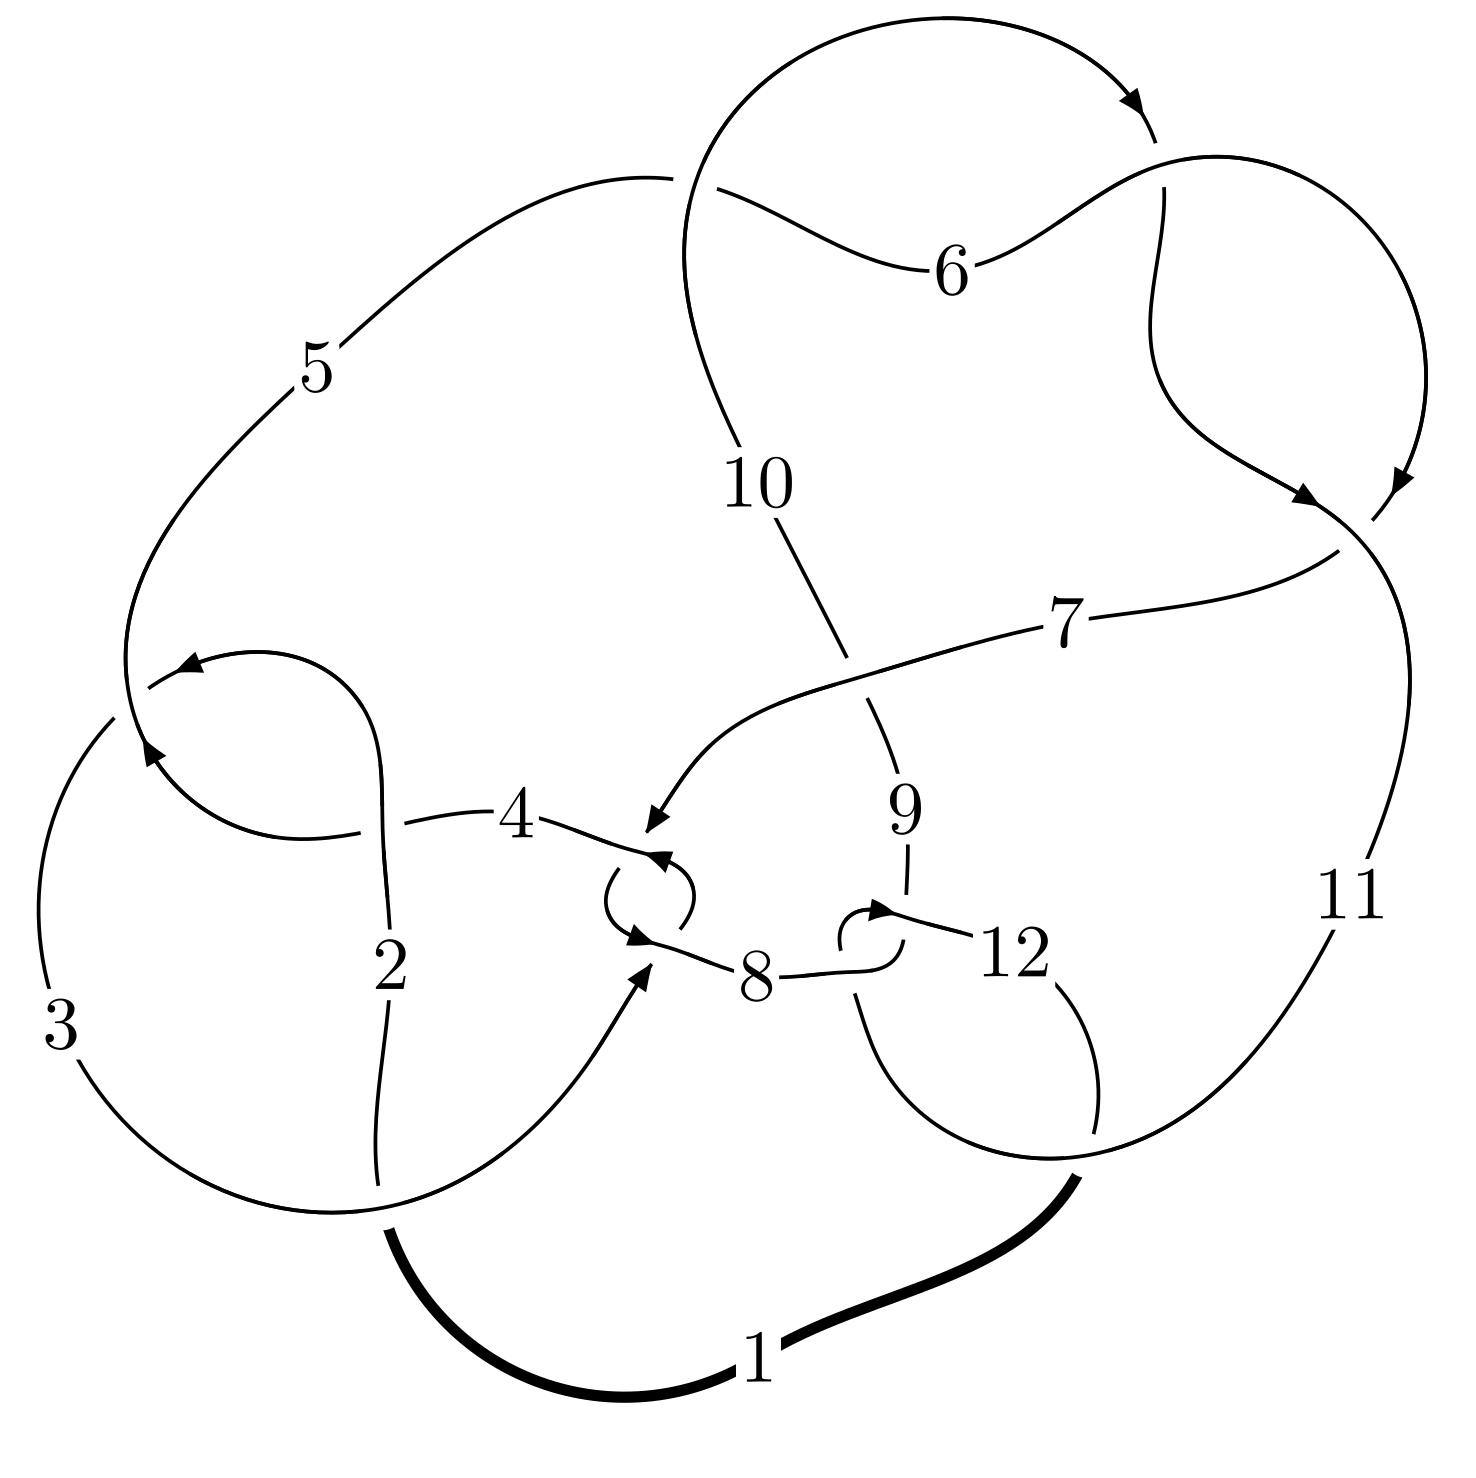
\includegraphics[width=112pt]{../../../GIT/diagram.site/Diagrams/png/2278_12n_0189.png}\\
\ \ \ A knot diagram\footnotemark}&
\allowdisplaybreaks
\textbf{Linearized knot diagam} \\
\cline{2-2}
 &
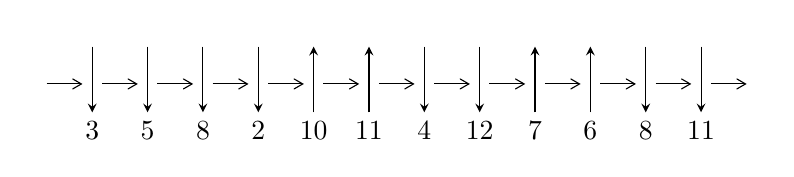
\begin{tikzpicture}[x=20pt, y=17pt]
	% nodes
	\node (C0) at (0, 0) {};
	\node (C1) at (1, 0) {};
	\node (C1U) at (1, +1) {};
	\node (C1D) at (1, -1) {3};

	\node (C2) at (2, 0) {};
	\node (C2U) at (2, +1) {};
	\node (C2D) at (2, -1) {5};

	\node (C3) at (3, 0) {};
	\node (C3U) at (3, +1) {};
	\node (C3D) at (3, -1) {8};

	\node (C4) at (4, 0) {};
	\node (C4U) at (4, +1) {};
	\node (C4D) at (4, -1) {2};

	\node (C5) at (5, 0) {};
	\node (C5U) at (5, +1) {};
	\node (C5D) at (5, -1) {10};

	\node (C6) at (6, 0) {};
	\node (C6U) at (6, +1) {};
	\node (C6D) at (6, -1) {11};

	\node (C7) at (7, 0) {};
	\node (C7U) at (7, +1) {};
	\node (C7D) at (7, -1) {4};

	\node (C8) at (8, 0) {};
	\node (C8U) at (8, +1) {};
	\node (C8D) at (8, -1) {12};

	\node (C9) at (9, 0) {};
	\node (C9U) at (9, +1) {};
	\node (C9D) at (9, -1) {7};

	\node (C10) at (10, 0) {};
	\node (C10U) at (10, +1) {};
	\node (C10D) at (10, -1) {6};

	\node (C11) at (11, 0) {};
	\node (C11U) at (11, +1) {};
	\node (C11D) at (11, -1) {8};

	\node (C12) at (12, 0) {};
	\node (C12U) at (12, +1) {};
	\node (C12D) at (12, -1) {11};
	\node (C13) at (13, 0) {};

	% arrows
	\draw[->,>={angle 60}]
	(C0) edge (C1) (C1) edge (C2) (C2) edge (C3) (C3) edge (C4) (C4) edge (C5) (C5) edge (C6) (C6) edge (C7) (C7) edge (C8) (C8) edge (C9) (C9) edge (C10) (C10) edge (C11) (C11) edge (C12) (C12) edge (C13) ;	\draw[->,>=stealth]
	(C1U) edge (C1D) (C2U) edge (C2D) (C3U) edge (C3D) (C4U) edge (C4D) (C5D) edge (C5U) (C6D) edge (C6U) (C7U) edge (C7D) (C8U) edge (C8D) (C9D) edge (C9U) (C10D) edge (C10U) (C11U) edge (C11D) (C12U) edge (C12D) ;
	\end{tikzpicture} \\
\hhline{~~} \\& 
\textbf{Solving Sequence} \\ \cline{2-2} 
 &
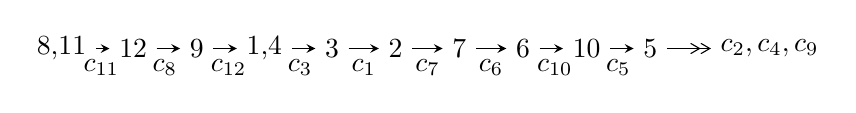
\begin{tikzpicture}[x=23pt, y=7pt]
	% node
	\node (A0) at (-1/8, 0) {8,11};
	\node (A1) at (1, 0) {12};
	\node (A2) at (2, 0) {9};
	\node (A3) at (49/16, 0) {1,4};
	\node (A4) at (33/8, 0) {3};
	\node (A5) at (41/8, 0) {2};
	\node (A6) at (49/8, 0) {7};
	\node (A7) at (57/8, 0) {6};
	\node (A8) at (65/8, 0) {10};
	\node (A9) at (73/8, 0) {5};
	\node (C1) at (1/2, -1) {$c_{11}$};
	\node (C2) at (3/2, -1) {$c_{8}$};
	\node (C3) at (5/2, -1) {$c_{12}$};
	\node (C4) at (29/8, -1) {$c_{3}$};
	\node (C5) at (37/8, -1) {$c_{1}$};
	\node (C6) at (45/8, -1) {$c_{7}$};
	\node (C7) at (53/8, -1) {$c_{6}$};
	\node (C8) at (61/8, -1) {$c_{10}$};
	\node (C9) at (69/8, -1) {$c_{5}$};
	\node (A10) at (11, 0) {$c_{2},c_{4},c_{9}$};

	% edge
	\draw[->,>=stealth]	
	(A0) edge (A1) (A1) edge (A2) (A2) edge (A3) (A3) edge (A4) (A4) edge (A5) (A5) edge (A6) (A6) edge (A7) (A7) edge (A8) (A8) edge (A9) ;
	\draw[->>,>={angle 60}]	
	(A9) edge (A10);
\end{tikzpicture} \\ 

\end{tabular} \\

\footnotetext{
The image of knot diagram is generated by the software ``\textbf{Draw programme}" developed by Andrew Bartholomew(\url{http://www.layer8.co.uk/maths/draw/index.htm\#Running-draw}), where we modified some parts for our purpose(\url{https://github.com/CATsTAILs/LinksPainter}).
}\phantom \\ \newline 
\centering \textbf{Ideals for irreducible components\footnotemark of $X_{\text{par}}$} 
 
\begin{align*}
I^u_{1}&=\langle 
2.49444\times10^{61} u^{47}+5.42508\times10^{61} u^{46}+\cdots+2.55281\times10^{62} b-1.56879\times10^{62},\\
\phantom{I^u_{1}}&\phantom{= \langle  }-4.23145\times10^{61} u^{47}-5.04595\times10^{62} u^{46}+\cdots+3.57394\times10^{63} a-9.28768\times10^{63},\\
\phantom{I^u_{1}}&\phantom{= \langle  }u^{48}+4 u^{47}+\cdots+59 u-7\rangle \\
I^u_{2}&=\langle 
-2 a^2 b+b^2-2 b a-2 a^2-4 b- a-3,\;a^3+a^2+2 a+1,\;u-1\rangle \\
I^u_{3}&=\langle 
- a^2+b- a-2,\;a^3+a^2+2 a+1,\;u+1\rangle \\
\\
\end{align*}
\raggedright * 3 irreducible components of $\dim_{\mathbb{C}}=0$, with total 57 representations.\\
\footnotetext{All coefficients of polynomials are rational numbers. But the coefficients are sometimes approximated in decimal forms when there is not enough margin.}
\newpage
\renewcommand{\arraystretch}{1}
\centering \section*{I. $I^u_{1}= \langle 2.49\times10^{61} u^{47}+5.43\times10^{61} u^{46}+\cdots+2.55\times10^{62} b-1.57\times10^{62},\;-4.23\times10^{61} u^{47}-5.05\times10^{62} u^{46}+\cdots+3.57\times10^{63} a-9.29\times10^{63},\;u^{48}+4 u^{47}+\cdots+59 u-7 \rangle$}
\flushleft \textbf{(i) Arc colorings}\\
\begin{tabular}{m{7pt} m{180pt} m{7pt} m{180pt} }
\flushright $a_{8}=$&$\begin{pmatrix}0\\u\end{pmatrix}$ \\
\flushright $a_{11}=$&$\begin{pmatrix}1\\0\end{pmatrix}$ \\
\flushright $a_{12}=$&$\begin{pmatrix}1\\u^2\end{pmatrix}$ \\
\flushright $a_{9}=$&$\begin{pmatrix}- u\\- u^3+u\end{pmatrix}$ \\
\flushright $a_{1}=$&$\begin{pmatrix}- u^2+1\\u^2\end{pmatrix}$ \\
\flushright $a_{4}=$&$\begin{pmatrix}0.0118397 u^{47}+0.141187 u^{46}+\cdots+28.4662 u+2.59872\\-0.0977134 u^{47}-0.212514 u^{46}+\cdots-12.5106 u+0.614532\end{pmatrix}$ \\
\flushright $a_{3}=$&$\begin{pmatrix}0.0118397 u^{47}+0.141187 u^{46}+\cdots+28.4662 u+2.59872\\-0.0177507 u^{47}+0.0119124 u^{46}+\cdots-7.05758 u-0.0422666\end{pmatrix}$ \\
\flushright $a_{2}=$&$\begin{pmatrix}-0.0759396 u^{47}-0.266607 u^{46}+\cdots-5.41635 u-1.07005\\-0.0304639 u^{47}-0.113488 u^{46}+\cdots+3.98647 u+0.0378137\end{pmatrix}$ \\
\flushright $a_{7}=$&$\begin{pmatrix}-0.135632 u^{47}-0.469213 u^{46}+\cdots+8.97335 u+2.53780\\-0.0896845 u^{47}-0.258891 u^{46}+\cdots+1.36877 u-0.441443\end{pmatrix}$ \\
\flushright $a_{6}=$&$\begin{pmatrix}-0.0459476 u^{47}-0.210322 u^{46}+\cdots+7.60458 u+2.97924\\-0.0896845 u^{47}-0.258891 u^{46}+\cdots+1.36877 u-0.441443\end{pmatrix}$ \\
\flushright $a_{10}=$&$\begin{pmatrix}0.157505 u^{47}+0.559805 u^{46}+\cdots+0.744089 u-1.23298\\0.0268891 u^{47}-0.0213891 u^{46}+\cdots+0.825649 u-0.103367\end{pmatrix}$ \\
\flushright $a_{5}=$&$\begin{pmatrix}0.0759396 u^{47}+0.266607 u^{46}+\cdots+5.41635 u+1.07005\\0.0604385 u^{47}+0.190773 u^{46}+\cdots-4.38559 u+0.332492\end{pmatrix}$\\&\end{tabular}
\flushleft \textbf{(ii) Obstruction class $= -1$}\\~\\
\flushleft \textbf{(iii) Cusp Shapes $= -0.523196 u^{47}-1.69630 u^{46}+\cdots-33.3905 u-3.88072$}\\~\\
\newpage\renewcommand{\arraystretch}{1}
\flushleft \textbf{(iv) u-Polynomials at the component}\newline \\
\begin{tabular}{m{50pt}|m{274pt}}
Crossings & \hspace{64pt}u-Polynomials at each crossing \\
\hline $$\begin{aligned}c_{1}\end{aligned}$$&$\begin{aligned}
&u^{48}+28 u^{47}+\cdots+2 u+1
\end{aligned}$\\
\hline $$\begin{aligned}c_{2},c_{4}\end{aligned}$$&$\begin{aligned}
&u^{48}-4 u^{47}+\cdots+2 u+1
\end{aligned}$\\
\hline $$\begin{aligned}c_{3},c_{7}\end{aligned}$$&$\begin{aligned}
&u^{48}+2 u^{47}+\cdots+8 u-1
\end{aligned}$\\
\hline $$\begin{aligned}c_{5},c_{6},c_{10}\end{aligned}$$&$\begin{aligned}
&u^{48}-3 u^{47}+\cdots-8 u-8
\end{aligned}$\\
\hline $$\begin{aligned}c_{8},c_{11}\end{aligned}$$&$\begin{aligned}
&u^{48}+4 u^{47}+\cdots+59 u-7
\end{aligned}$\\
\hline $$\begin{aligned}c_{9}\end{aligned}$$&$\begin{aligned}
&u^{48}+9 u^{47}+\cdots-6632 u-1192
\end{aligned}$\\
\hline $$\begin{aligned}c_{12}\end{aligned}$$&$\begin{aligned}
&u^{48}+54 u^{47}+\cdots+4853 u+49
\end{aligned}$\\
\hline
\end{tabular}\\~\\
\newpage\renewcommand{\arraystretch}{1}
\flushleft \textbf{(v) Riley Polynomials at the component}\newline \\
\begin{tabular}{m{50pt}|m{274pt}}
Crossings & \hspace{64pt}Riley Polynomials at each crossing \\
\hline $$\begin{aligned}c_{1}\end{aligned}$$&$\begin{aligned}
&y^{48}-12 y^{47}+\cdots-250 y+1
\end{aligned}$\\
\hline $$\begin{aligned}c_{2},c_{4}\end{aligned}$$&$\begin{aligned}
&y^{48}-28 y^{47}+\cdots-2 y+1
\end{aligned}$\\
\hline $$\begin{aligned}c_{3},c_{7}\end{aligned}$$&$\begin{aligned}
&y^{48}+12 y^{47}+\cdots-42 y+1
\end{aligned}$\\
\hline $$\begin{aligned}c_{5},c_{6},c_{10}\end{aligned}$$&$\begin{aligned}
&y^{48}-41 y^{47}+\cdots-1984 y+64
\end{aligned}$\\
\hline $$\begin{aligned}c_{8},c_{11}\end{aligned}$$&$\begin{aligned}
&y^{48}-54 y^{47}+\cdots-4853 y+49
\end{aligned}$\\
\hline $$\begin{aligned}c_{9}\end{aligned}$$&$\begin{aligned}
&y^{48}+43 y^{47}+\cdots-58172992 y+1420864
\end{aligned}$\\
\hline $$\begin{aligned}c_{12}\end{aligned}$$&$\begin{aligned}
&y^{48}-110 y^{47}+\cdots-30351829 y+2401
\end{aligned}$\\
\hline
\end{tabular}\\~\\
\newpage\flushleft \textbf{(vi) Complex Volumes and Cusp Shapes}
$$\begin{array}{c|c|c}  
\text{Solutions to }I^u_{1}& \I (\text{vol} + \sqrt{-1}CS) & \text{Cusp shape}\\
 \hline 
\begin{aligned}
u &= \phantom{-}1.03474\phantom{ +0.000000I} \\
a &= -0.149518\phantom{ +0.000000I} \\
b &= \phantom{-}15.9108\phantom{ +0.000000I}\end{aligned}
 & \phantom{-}1.67136\phantom{ +0.000000I} & -181.820\phantom{ +0.000000I} \\ \hline\begin{aligned}
u &= -1.10270\phantom{ +0.000000I} \\
a &= \phantom{-}0.558674\phantom{ +0.000000I} \\
b &= -1.21115\phantom{ +0.000000I}\end{aligned}
 & -2.51979\phantom{ +0.000000I} & \phantom{-}7.01870\phantom{ +0.000000I} \\ \hline\begin{aligned}
u &= \phantom{-}0.402947 + 0.795966 I \\
a &= -1.253190 + 0.172447 I \\
b &= \phantom{-}1.24412 - 0.98353 I\end{aligned}
 & \phantom{-}4.33668 - 4.44228 I & \phantom{-}2.15682 + 4.76767 I \\ \hline\begin{aligned}
u &= \phantom{-}0.402947 - 0.795966 I \\
a &= -1.253190 - 0.172447 I \\
b &= \phantom{-}1.24412 + 0.98353 I\end{aligned}
 & \phantom{-}4.33668 + 4.44228 I & \phantom{-}2.15682 - 4.76767 I \\ \hline\begin{aligned}
u &= \phantom{-}0.549733 + 0.682678 I \\
a &= \phantom{-}0.009774 - 1.180920 I \\
b &= \phantom{-}1.026340 - 0.304021 I\end{aligned}
 & \phantom{-}0.44919 - 3.43575 I & -2.94781 + 4.14151 I \\ \hline\begin{aligned}
u &= \phantom{-}0.549733 - 0.682678 I \\
a &= \phantom{-}0.009774 + 1.180920 I \\
b &= \phantom{-}1.026340 + 0.304021 I\end{aligned}
 & \phantom{-}0.44919 + 3.43575 I & -2.94781 - 4.14151 I \\ \hline\begin{aligned}
u &= \phantom{-}0.607419 + 0.971287 I \\
a &= -0.314066 - 0.576245 I \\
b &= \phantom{-}0.709420 + 0.166838 I\end{aligned}
 & \phantom{-}0.79074 + 2.62631 I & \phantom{-0.000000 } 0. - 8.02541 I \\ \hline\begin{aligned}
u &= \phantom{-}0.607419 - 0.971287 I \\
a &= -0.314066 + 0.576245 I \\
b &= \phantom{-}0.709420 - 0.166838 I\end{aligned}
 & \phantom{-}0.79074 - 2.62631 I & \phantom{-0.000000 -}0. + 8.02541 I \\ \hline\begin{aligned}
u &= \phantom{-}0.529099 + 1.030160 I \\
a &= \phantom{-}1.023660 - 0.202973 I \\
b &= -1.33032 + 0.89512 I\end{aligned}
 & \phantom{-}1.27119 - 9.09207 I & \phantom{-0.000000 -}0. + 7.97032 I \\ \hline\begin{aligned}
u &= \phantom{-}0.529099 - 1.030160 I \\
a &= \phantom{-}1.023660 + 0.202973 I \\
b &= -1.33032 - 0.89512 I\end{aligned}
 & \phantom{-}1.27119 + 9.09207 I & \phantom{-0.000000 } 0. - 7.97032 I\\
 \hline 
 \end{array}$$\newpage$$\begin{array}{c|c|c}  
\text{Solutions to }I^u_{1}& \I (\text{vol} + \sqrt{-1}CS) & \text{Cusp shape}\\
 \hline 
\begin{aligned}
u &= \phantom{-}0.606029 + 0.575291 I \\
a &= \phantom{-}1.095020 + 0.107629 I \\
b &= -1.62264 + 1.09670 I\end{aligned}
 & \phantom{-}0.227251 - 0.982213 I & -2.97456 + 4.05134 I \\ \hline\begin{aligned}
u &= \phantom{-}0.606029 - 0.575291 I \\
a &= \phantom{-}1.095020 - 0.107629 I \\
b &= -1.62264 - 1.09670 I\end{aligned}
 & \phantom{-}0.227251 + 0.982213 I & -2.97456 - 4.05134 I \\ \hline\begin{aligned}
u &= \phantom{-}0.717418 + 0.339614 I \\
a &= -0.411980 + 0.676361 I \\
b &= -1.010750 - 0.101614 I\end{aligned}
 & \phantom{-}3.05609 + 0.03450 I & \phantom{-}1.61725 - 0.04014 I \\ \hline\begin{aligned}
u &= \phantom{-}0.717418 - 0.339614 I \\
a &= -0.411980 - 0.676361 I \\
b &= -1.010750 + 0.101614 I\end{aligned}
 & \phantom{-}3.05609 - 0.03450 I & \phantom{-}1.61725 + 0.04014 I \\ \hline\begin{aligned}
u &= \phantom{-}0.774869 + 0.143809 I \\
a &= \phantom{-}0.06554 - 1.56635 I \\
b &= \phantom{-}0.115818 - 0.297169 I\end{aligned}
 & \phantom{-}1.81458 + 2.58829 I & \phantom{-}4.64199 + 0.62738 I \\ \hline\begin{aligned}
u &= \phantom{-}0.774869 - 0.143809 I \\
a &= \phantom{-}0.06554 + 1.56635 I \\
b &= \phantom{-}0.115818 + 0.297169 I\end{aligned}
 & \phantom{-}1.81458 - 2.58829 I & \phantom{-}4.64199 - 0.62738 I \\ \hline\begin{aligned}
u &= -0.705342 + 0.225017 I \\
a &= \phantom{-}0.374486 + 0.783406 I \\
b &= -0.02299 + 1.57993 I\end{aligned}
 & -2.89686 + 0.77640 I & -12.15233 + 3.40612 I \\ \hline\begin{aligned}
u &= -0.705342 - 0.225017 I \\
a &= \phantom{-}0.374486 - 0.783406 I \\
b &= -0.02299 - 1.57993 I\end{aligned}
 & -2.89686 - 0.77640 I & -12.15233 - 3.40612 I \\ \hline\begin{aligned}
u &= \phantom{-}0.701884\phantom{ +0.000000I} \\
a &= -0.734892\phantom{ +0.000000I} \\
b &= -1.24205\phantom{ +0.000000I}\end{aligned}
 & \phantom{-}3.11349\phantom{ +0.000000I} & \phantom{-}3.07850\phantom{ +0.000000I} \\ \hline\begin{aligned}
u &= -0.856659 + 0.985459 I \\
a &= \phantom{-}0.636632 + 0.001328 I \\
b &= -0.672001 - 0.732654 I\end{aligned}
 & -2.80642 + 4.10771 I & \phantom{-0.000000 } 0\\
 \hline 
 \end{array}$$\newpage$$\begin{array}{c|c|c}  
\text{Solutions to }I^u_{1}& \I (\text{vol} + \sqrt{-1}CS) & \text{Cusp shape}\\
 \hline 
\begin{aligned}
u &= -0.856659 - 0.985459 I \\
a &= \phantom{-}0.636632 - 0.001328 I \\
b &= -0.672001 + 0.732654 I\end{aligned}
 & -2.80642 - 4.10771 I & \phantom{-0.000000 } 0 \\ \hline\begin{aligned}
u &= -1.312340 + 0.022176 I \\
a &= \phantom{-}0.159774 - 1.198270 I \\
b &= -0.14705 - 1.53594 I\end{aligned}
 & \phantom{-}3.83816 + 3.33221 I & \phantom{-0.000000 } 0 \\ \hline\begin{aligned}
u &= -1.312340 - 0.022176 I \\
a &= \phantom{-}0.159774 + 1.198270 I \\
b &= -0.14705 + 1.53594 I\end{aligned}
 & \phantom{-}3.83816 - 3.33221 I & \phantom{-0.000000 } 0 \\ \hline\begin{aligned}
u &= -0.382101 + 0.518429 I \\
a &= -1.066440 - 0.036820 I \\
b &= \phantom{-}0.434772 + 0.642582 I\end{aligned}
 & -0.164421 + 1.292600 I & -1.96598 - 5.14574 I \\ \hline\begin{aligned}
u &= -0.382101 - 0.518429 I \\
a &= -1.066440 + 0.036820 I \\
b &= \phantom{-}0.434772 - 0.642582 I\end{aligned}
 & -0.164421 - 1.292600 I & -1.96598 + 5.14574 I \\ \hline\begin{aligned}
u &= -1.52813 + 0.03469 I \\
a &= \phantom{-}0.749487 + 0.430849 I \\
b &= -0.082283 + 0.460779 I\end{aligned}
 & -3.85416 + 1.06668 I & \phantom{-0.000000 } 0 \\ \hline\begin{aligned}
u &= -1.52813 - 0.03469 I \\
a &= \phantom{-}0.749487 - 0.430849 I \\
b &= -0.082283 - 0.460779 I\end{aligned}
 & -3.85416 - 1.06668 I & \phantom{-0.000000 } 0 \\ \hline\begin{aligned}
u &= \phantom{-}1.49504 + 0.38475 I \\
a &= \phantom{-}0.007881 + 0.362733 I \\
b &= -0.372006 - 0.161707 I\end{aligned}
 & \phantom{-}2.74848 + 0.89020 I & \phantom{-0.000000 } 0 \\ \hline\begin{aligned}
u &= \phantom{-}1.49504 - 0.38475 I \\
a &= \phantom{-}0.007881 - 0.362733 I \\
b &= -0.372006 + 0.161707 I\end{aligned}
 & \phantom{-}2.74848 - 0.89020 I & \phantom{-0.000000 } 0 \\ \hline\begin{aligned}
u &= -1.52900 + 0.29105 I \\
a &= \phantom{-}0.706345 - 0.671808 I \\
b &= -1.06205 - 1.60612 I\end{aligned}
 & -2.00876 + 8.44086 I & \phantom{-0.000000 } 0\\
 \hline 
 \end{array}$$\newpage$$\begin{array}{c|c|c}  
\text{Solutions to }I^u_{1}& \I (\text{vol} + \sqrt{-1}CS) & \text{Cusp shape}\\
 \hline 
\begin{aligned}
u &= -1.52900 - 0.29105 I \\
a &= \phantom{-}0.706345 + 0.671808 I \\
b &= -1.06205 + 1.60612 I\end{aligned}
 & -2.00876 - 8.44086 I & \phantom{-0.000000 } 0 \\ \hline\begin{aligned}
u &= \phantom{-}1.55775 + 0.15557 I \\
a &= \phantom{-}0.721994 + 0.568337 I \\
b &= -0.497955 + 1.196310 I\end{aligned}
 & -6.88003 - 3.75478 I & \phantom{-0.000000 } 0 \\ \hline\begin{aligned}
u &= \phantom{-}1.55775 - 0.15557 I \\
a &= \phantom{-}0.721994 - 0.568337 I \\
b &= -0.497955 - 1.196310 I\end{aligned}
 & -6.88003 + 3.75478 I & \phantom{-0.000000 } 0 \\ \hline\begin{aligned}
u &= -1.58783 + 0.13072 I \\
a &= -0.527458 + 0.690762 I \\
b &= \phantom{-}0.89707 + 1.86682 I\end{aligned}
 & -7.23928 + 3.38751 I & \phantom{-0.000000 } 0 \\ \hline\begin{aligned}
u &= -1.58783 - 0.13072 I \\
a &= -0.527458 - 0.690762 I \\
b &= \phantom{-}0.89707 - 1.86682 I\end{aligned}
 & -7.23928 - 3.38751 I & \phantom{-0.000000 } 0 \\ \hline\begin{aligned}
u &= -1.58112 + 0.20855 I \\
a &= -0.673201 - 0.601686 I \\
b &= -0.115011 - 0.480919 I\end{aligned}
 & -6.71802 + 6.70728 I & \phantom{-0.000000 } 0 \\ \hline\begin{aligned}
u &= -1.58112 - 0.20855 I \\
a &= -0.673201 + 0.601686 I \\
b &= -0.115011 + 0.480919 I\end{aligned}
 & -6.71802 - 6.70728 I & \phantom{-0.000000 } 0 \\ \hline\begin{aligned}
u &= \phantom{-}1.61634 + 0.04594 I \\
a &= -0.607271 + 0.648913 I \\
b &= \phantom{-}0.278472 + 1.264590 I\end{aligned}
 & -10.99530 - 1.69093 I & \phantom{-0.000000 } 0 \\ \hline\begin{aligned}
u &= \phantom{-}1.61634 - 0.04594 I \\
a &= -0.607271 - 0.648913 I \\
b &= \phantom{-}0.278472 - 1.264590 I\end{aligned}
 & -10.99530 + 1.69093 I & \phantom{-0.000000 } 0 \\ \hline\begin{aligned}
u &= -1.59092 + 0.39585 I \\
a &= -0.731570 + 0.550707 I \\
b &= \phantom{-}1.26602 + 1.60368 I\end{aligned}
 & -5.5392 + 14.3589 I & \phantom{-0.000000 } 0\\
 \hline 
 \end{array}$$\newpage$$\begin{array}{c|c|c}  
\text{Solutions to }I^u_{1}& \I (\text{vol} + \sqrt{-1}CS) & \text{Cusp shape}\\
 \hline 
\begin{aligned}
u &= -1.59092 - 0.39585 I \\
a &= -0.731570 - 0.550707 I \\
b &= \phantom{-}1.26602 - 1.60368 I\end{aligned}
 & -5.5392 - 14.3589 I & \phantom{-0.000000 } 0 \\ \hline\begin{aligned}
u &= \phantom{-}1.68738 + 0.31170 I \\
a &= -0.685391 - 0.453228 I \\
b &= \phantom{-}0.64974 - 1.33823 I\end{aligned}
 & -11.1104 - 9.0785 I & \phantom{-0.000000 } 0 \\ \hline\begin{aligned}
u &= \phantom{-}1.68738 - 0.31170 I \\
a &= -0.685391 + 0.453228 I \\
b &= \phantom{-}0.64974 + 1.33823 I\end{aligned}
 & -11.1104 + 9.0785 I & \phantom{-0.000000 } 0 \\ \hline\begin{aligned}
u &= -1.74551 + 0.16291 I \\
a &= -0.577118 + 0.344131 I \\
b &= \phantom{-}0.165920 + 0.739123 I\end{aligned}
 & -8.76602 + 2.97970 I & \phantom{-0.000000 } 0 \\ \hline\begin{aligned}
u &= -1.74551 - 0.16291 I \\
a &= -0.577118 - 0.344131 I \\
b &= \phantom{-}0.165920 - 0.739123 I\end{aligned}
 & -8.76602 - 2.97970 I & \phantom{-0.000000 } 0 \\ \hline\begin{aligned}
u &= -0.088616 + 0.165371 I \\
a &= -5.53925 + 3.96896 I \\
b &= \phantom{-}0.242833 - 1.027870 I\end{aligned}
 & \phantom{-}7.99255 - 2.76208 I & \phantom{-}5.58674 + 2.99226 I \\ \hline\begin{aligned}
u &= -0.088616 - 0.165371 I \\
a &= -5.53925 - 3.96896 I \\
b &= \phantom{-}0.242833 + 1.027870 I\end{aligned}
 & \phantom{-}7.99255 + 2.76208 I & \phantom{-}5.58674 - 2.99226 I \\ \hline\begin{aligned}
u &= \phantom{-}0.0931699\phantom{ +0.000000I} \\
a &= \phantom{-}5.14127\phantom{ +0.000000I} \\
b &= -0.648531\phantom{ +0.000000I}\end{aligned}
 & -1.24876\phantom{ +0.000000I} & -7.95330\phantom{ +0.000000I}\\
 \hline 
 \end{array}$$\newpage\newpage\renewcommand{\arraystretch}{1}
\centering \section*{II. $I^u_{2}= \langle -2 a^2 b+b^2-2 b a-2 a^2-4 b- a-3,\;a^3+a^2+2 a+1,\;u-1 \rangle$}
\flushleft \textbf{(i) Arc colorings}\\
\begin{tabular}{m{7pt} m{180pt} m{7pt} m{180pt} }
\flushright $a_{8}=$&$\begin{pmatrix}0\\1\end{pmatrix}$ \\
\flushright $a_{11}=$&$\begin{pmatrix}1\\0\end{pmatrix}$ \\
\flushright $a_{12}=$&$\begin{pmatrix}1\\1\end{pmatrix}$ \\
\flushright $a_{9}=$&$\begin{pmatrix}-1\\0\end{pmatrix}$ \\
\flushright $a_{1}=$&$\begin{pmatrix}0\\1\end{pmatrix}$ \\
\flushright $a_{4}=$&$\begin{pmatrix}a\\b\end{pmatrix}$ \\
\flushright $a_{3}=$&$\begin{pmatrix}a\\b- a\end{pmatrix}$ \\
\flushright $a_{2}=$&$\begin{pmatrix}- a^2\\- b a+a^2+1\end{pmatrix}$ \\
\flushright $a_{7}=$&$\begin{pmatrix}a^2\\b a+1\end{pmatrix}$ \\
\flushright $a_{6}=$&$\begin{pmatrix}- b a+a^2-1\\b a+1\end{pmatrix}$ \\
\flushright $a_{10}=$&$\begin{pmatrix}- a^2 b-2 b a+a^2- b-1\\2\end{pmatrix}$ \\
\flushright $a_{5}=$&$\begin{pmatrix}- a^2\\- b a-1\end{pmatrix}$\\&\end{tabular}
\flushleft \textbf{(ii) Obstruction class $= 1$}\\~\\
\flushleft \textbf{(iii) Cusp Shapes $= -4 a^2-4 a-8$}\\~\\
\newpage\renewcommand{\arraystretch}{1}
\flushleft \textbf{(iv) u-Polynomials at the component}\newline \\
\begin{tabular}{m{50pt}|m{274pt}}
Crossings & \hspace{64pt}u-Polynomials at each crossing \\
\hline $$\begin{aligned}c_{1},c_{7}\end{aligned}$$&$\begin{aligned}
&(u^3- u^2+2 u-1)^2
\end{aligned}$\\
\hline $$\begin{aligned}c_{2}\end{aligned}$$&$\begin{aligned}
&(u^3+u^2-1)^2
\end{aligned}$\\
\hline $$\begin{aligned}c_{3}\end{aligned}$$&$\begin{aligned}
&(u^3+u^2+2 u+1)^2
\end{aligned}$\\
\hline $$\begin{aligned}c_{4}\end{aligned}$$&$\begin{aligned}
&(u^3- u^2+1)^2
\end{aligned}$\\
\hline $$\begin{aligned}c_{5},c_{6},c_{9}\\c_{10}\end{aligned}$$&$\begin{aligned}
&(u^2-2)^3
\end{aligned}$\\
\hline $$\begin{aligned}c_{8},c_{12}\end{aligned}$$&$\begin{aligned}
&(u+1)^6
\end{aligned}$\\
\hline $$\begin{aligned}c_{11}\end{aligned}$$&$\begin{aligned}
&(u-1)^6
\end{aligned}$\\
\hline
\end{tabular}\\~\\
\newpage\renewcommand{\arraystretch}{1}
\flushleft \textbf{(v) Riley Polynomials at the component}\newline \\
\begin{tabular}{m{50pt}|m{274pt}}
Crossings & \hspace{64pt}Riley Polynomials at each crossing \\
\hline $$\begin{aligned}c_{1},c_{3},c_{7}\end{aligned}$$&$\begin{aligned}
&(y^3+3 y^2+2 y-1)^2
\end{aligned}$\\
\hline $$\begin{aligned}c_{2},c_{4}\end{aligned}$$&$\begin{aligned}
&(y^3- y^2+2 y-1)^2
\end{aligned}$\\
\hline $$\begin{aligned}c_{5},c_{6},c_{9}\\c_{10}\end{aligned}$$&$\begin{aligned}
&(y-2)^6
\end{aligned}$\\
\hline $$\begin{aligned}c_{8},c_{11},c_{12}\end{aligned}$$&$\begin{aligned}
&(y-1)^6
\end{aligned}$\\
\hline
\end{tabular}\\~\\
\newpage\flushleft \textbf{(vi) Complex Volumes and Cusp Shapes}
$$\begin{array}{c|c|c}  
\text{Solutions to }I^u_{2}& \I (\text{vol} + \sqrt{-1}CS) & \text{Cusp shape}\\
 \hline 
\begin{aligned}
u &= \phantom{-}1.00000\phantom{ +0.000000I} \\
a &= -0.215080 + 1.307140 I \\
b &= -0.050766 - 0.308532 I\end{aligned}
 & \phantom{-}6.31400 + 2.82812 I & -0.49024 - 2.97945 I \\ \hline\begin{aligned}
u &= \phantom{-}1.00000\phantom{ +0.000000I} \\
a &= -0.215080 + 1.307140 I \\
b &= \phantom{-}0.29589 + 1.79826 I\end{aligned}
 & \phantom{-}6.31400 + 2.82812 I & -0.49024 - 2.97945 I \\ \hline\begin{aligned}
u &= \phantom{-}1.00000\phantom{ +0.000000I} \\
a &= -0.215080 - 1.307140 I \\
b &= -0.050766 + 0.308532 I\end{aligned}
 & \phantom{-}6.31400 - 2.82812 I & -0.49024 + 2.97945 I \\ \hline\begin{aligned}
u &= \phantom{-}1.00000\phantom{ +0.000000I} \\
a &= -0.215080 - 1.307140 I \\
b &= \phantom{-}0.29589 - 1.79826 I\end{aligned}
 & \phantom{-}6.31400 - 2.82812 I & -0.49024 + 2.97945 I \\ \hline\begin{aligned}
u &= \phantom{-}1.00000\phantom{ +0.000000I} \\
a &= -0.569840\phantom{ +0.000000I} \\
b &= -0.726894\phantom{ +0.000000I}\end{aligned}
 & \phantom{-}2.17641\phantom{ +0.000000I} & -7.01950\phantom{ +0.000000I} \\ \hline\begin{aligned}
u &= \phantom{-}1.00000\phantom{ +0.000000I} \\
a &= -0.569840\phantom{ +0.000000I} \\
b &= \phantom{-}4.23665\phantom{ +0.000000I}\end{aligned}
 & \phantom{-}2.17641\phantom{ +0.000000I} & -7.01950\phantom{ +0.000000I}\\
 \hline 
 \end{array}$$\newpage\newpage\renewcommand{\arraystretch}{1}
\centering \section*{III. $I^u_{3}= \langle - a^2+b- a-2,\;a^3+a^2+2 a+1,\;u+1 \rangle$}
\flushleft \textbf{(i) Arc colorings}\\
\begin{tabular}{m{7pt} m{180pt} m{7pt} m{180pt} }
\flushright $a_{8}=$&$\begin{pmatrix}0\\-1\end{pmatrix}$ \\
\flushright $a_{11}=$&$\begin{pmatrix}1\\0\end{pmatrix}$ \\
\flushright $a_{12}=$&$\begin{pmatrix}1\\1\end{pmatrix}$ \\
\flushright $a_{9}=$&$\begin{pmatrix}1\\0\end{pmatrix}$ \\
\flushright $a_{1}=$&$\begin{pmatrix}0\\1\end{pmatrix}$ \\
\flushright $a_{4}=$&$\begin{pmatrix}a\\a^2+a+2\end{pmatrix}$ \\
\flushright $a_{3}=$&$\begin{pmatrix}a\\a^2+2\end{pmatrix}$ \\
\flushright $a_{2}=$&$\begin{pmatrix}- a^2\\a^2+2\end{pmatrix}$ \\
\flushright $a_{7}=$&$\begin{pmatrix}- a^2\\0\end{pmatrix}$ \\
\flushright $a_{6}=$&$\begin{pmatrix}- a^2\\0\end{pmatrix}$ \\
\flushright $a_{10}=$&$\begin{pmatrix}1\\0\end{pmatrix}$ \\
\flushright $a_{5}=$&$\begin{pmatrix}- a^2\\0\end{pmatrix}$\\&\end{tabular}
\flushleft \textbf{(ii) Obstruction class $= 1$}\\~\\
\flushleft \textbf{(iii) Cusp Shapes $= -12 a^2-10 a-32$}\\~\\
\newpage\renewcommand{\arraystretch}{1}
\flushleft \textbf{(iv) u-Polynomials at the component}\newline \\
\begin{tabular}{m{50pt}|m{274pt}}
Crossings & \hspace{64pt}u-Polynomials at each crossing \\
\hline $$\begin{aligned}c_{1},c_{3}\end{aligned}$$&$\begin{aligned}
&u^3- u^2+2 u-1
\end{aligned}$\\
\hline $$\begin{aligned}c_{2}\end{aligned}$$&$\begin{aligned}
&u^3+u^2-1
\end{aligned}$\\
\hline $$\begin{aligned}c_{4}\end{aligned}$$&$\begin{aligned}
&u^3- u^2+1
\end{aligned}$\\
\hline $$\begin{aligned}c_{5},c_{6},c_{9}\\c_{10}\end{aligned}$$&$\begin{aligned}
&u^3
\end{aligned}$\\
\hline $$\begin{aligned}c_{7}\end{aligned}$$&$\begin{aligned}
&u^3+u^2+2 u+1
\end{aligned}$\\
\hline $$\begin{aligned}c_{8}\end{aligned}$$&$\begin{aligned}
&(u-1)^3
\end{aligned}$\\
\hline $$\begin{aligned}c_{11},c_{12}\end{aligned}$$&$\begin{aligned}
&(u+1)^3
\end{aligned}$\\
\hline
\end{tabular}\\~\\
\newpage\renewcommand{\arraystretch}{1}
\flushleft \textbf{(v) Riley Polynomials at the component}\newline \\
\begin{tabular}{m{50pt}|m{274pt}}
Crossings & \hspace{64pt}Riley Polynomials at each crossing \\
\hline $$\begin{aligned}c_{1},c_{3},c_{7}\end{aligned}$$&$\begin{aligned}
&y^3+3 y^2+2 y-1
\end{aligned}$\\
\hline $$\begin{aligned}c_{2},c_{4}\end{aligned}$$&$\begin{aligned}
&y^3- y^2+2 y-1
\end{aligned}$\\
\hline $$\begin{aligned}c_{5},c_{6},c_{9}\\c_{10}\end{aligned}$$&$\begin{aligned}
&y^3
\end{aligned}$\\
\hline $$\begin{aligned}c_{8},c_{11},c_{12}\end{aligned}$$&$\begin{aligned}
&(y-1)^3
\end{aligned}$\\
\hline
\end{tabular}\\~\\
\newpage\flushleft \textbf{(vi) Complex Volumes and Cusp Shapes}
$$\begin{array}{c|c|c}  
\text{Solutions to }I^u_{3}& \I (\text{vol} + \sqrt{-1}CS) & \text{Cusp shape}\\
 \hline 
\begin{aligned}
u &= -1.00000\phantom{ +0.000000I} \\
a &= -0.215080 + 1.307140 I \\
b &= \phantom{-}0.122561 + 0.744862 I\end{aligned}
 & \phantom{-}1.37919 + 2.82812 I & -9.90089 - 6.32406 I \\ \hline\begin{aligned}
u &= -1.00000\phantom{ +0.000000I} \\
a &= -0.215080 - 1.307140 I \\
b &= \phantom{-}0.122561 - 0.744862 I\end{aligned}
 & \phantom{-}1.37919 - 2.82812 I & -9.90089 + 6.32406 I \\ \hline\begin{aligned}
u &= -1.00000\phantom{ +0.000000I} \\
a &= -0.569840\phantom{ +0.000000I} \\
b &= \phantom{-}1.75488\phantom{ +0.000000I}\end{aligned}
 & -2.75839\phantom{ +0.000000I} & -30.1980\phantom{ +0.000000I}\\
 \hline 
 \end{array}$$\newpage
\newpage\renewcommand{\arraystretch}{1}
\centering \section*{ IV. u-Polynomials}
\begin{tabular}{m{50pt}|m{274pt}}
Crossings & \hspace{64pt}u-Polynomials at each crossing \\
\hline $$\begin{aligned}c_{1}\end{aligned}$$&$\begin{aligned}
&((u^3- u^2+2 u-1)^3)(u^{48}+28 u^{47}+\cdots+2 u+1)
\end{aligned}$\\
\hline $$\begin{aligned}c_{2}\end{aligned}$$&$\begin{aligned}
&((u^3+u^2-1)^3)(u^{48}-4 u^{47}+\cdots+2 u+1)
\end{aligned}$\\
\hline $$\begin{aligned}c_{3}\end{aligned}$$&$\begin{aligned}
&(u^3- u^2+2 u-1)(u^3+u^2+2 u+1)^2(u^{48}+2 u^{47}+\cdots+8 u-1)
\end{aligned}$\\
\hline $$\begin{aligned}c_{4}\end{aligned}$$&$\begin{aligned}
&((u^3- u^2+1)^3)(u^{48}-4 u^{47}+\cdots+2 u+1)
\end{aligned}$\\
\hline $$\begin{aligned}c_{5},c_{6},c_{10}\end{aligned}$$&$\begin{aligned}
&u^3(u^2-2)^3(u^{48}-3 u^{47}+\cdots-8 u-8)
\end{aligned}$\\
\hline $$\begin{aligned}c_{7}\end{aligned}$$&$\begin{aligned}
&((u^3- u^2+2 u-1)^2)(u^3+u^2+2 u+1)(u^{48}+2 u^{47}+\cdots+8 u-1)
\end{aligned}$\\
\hline $$\begin{aligned}c_{8}\end{aligned}$$&$\begin{aligned}
&((u-1)^3)(u+1)^6(u^{48}+4 u^{47}+\cdots+59 u-7)
\end{aligned}$\\
\hline $$\begin{aligned}c_{9}\end{aligned}$$&$\begin{aligned}
&u^3(u^2-2)^3(u^{48}+9 u^{47}+\cdots-6632 u-1192)
\end{aligned}$\\
\hline $$\begin{aligned}c_{11}\end{aligned}$$&$\begin{aligned}
&((u-1)^6)(u+1)^3(u^{48}+4 u^{47}+\cdots+59 u-7)
\end{aligned}$\\
\hline $$\begin{aligned}c_{12}\end{aligned}$$&$\begin{aligned}
&((u+1)^9)(u^{48}+54 u^{47}+\cdots+4853 u+49)
\end{aligned}$\\
\hline
\end{tabular}\newpage\renewcommand{\arraystretch}{1}
\centering \section*{ V. Riley Polynomials}
\begin{tabular}{m{50pt}|m{274pt}}
Crossings & \hspace{64pt}Riley Polynomials at each crossing \\
\hline $$\begin{aligned}c_{1}\end{aligned}$$&$\begin{aligned}
&((y^3+3 y^2+2 y-1)^3)(y^{48}-12 y^{47}+\cdots-250 y+1)
\end{aligned}$\\
\hline $$\begin{aligned}c_{2},c_{4}\end{aligned}$$&$\begin{aligned}
&((y^3- y^2+2 y-1)^3)(y^{48}-28 y^{47}+\cdots-2 y+1)
\end{aligned}$\\
\hline $$\begin{aligned}c_{3},c_{7}\end{aligned}$$&$\begin{aligned}
&((y^3+3 y^2+2 y-1)^3)(y^{48}+12 y^{47}+\cdots-42 y+1)
\end{aligned}$\\
\hline $$\begin{aligned}c_{5},c_{6},c_{10}\end{aligned}$$&$\begin{aligned}
&y^3(y-2)^6(y^{48}-41 y^{47}+\cdots-1984 y+64)
\end{aligned}$\\
\hline $$\begin{aligned}c_{8},c_{11}\end{aligned}$$&$\begin{aligned}
&((y-1)^9)(y^{48}-54 y^{47}+\cdots-4853 y+49)
\end{aligned}$\\
\hline $$\begin{aligned}c_{9}\end{aligned}$$&$\begin{aligned}
&y^3(y-2)^6(y^{48}+43 y^{47}+\cdots-5.81730\times10^{7} y+1420864)
\end{aligned}$\\
\hline $$\begin{aligned}c_{12}\end{aligned}$$&$\begin{aligned}
&((y-1)^9)(y^{48}-110 y^{47}+\cdots-3.03518\times10^{7} y+2401)
\end{aligned}$\\
\hline
\end{tabular}
\vskip 2pc
\end{document}